% Taller RL — informe de 2 páginas. Compilar: pdflatex informe.tex (dos veces). Figuras en ./figuras/
\documentclass[10pt,a4paper]{article}
\usepackage[utf8]{inputenc}
\usepackage[T1]{fontenc}
\usepackage[spanish,es-noquoting,es-nodecimaldot]{babel}
\usepackage{lmodern,microtype}
\usepackage[a4paper,top=1.3cm,bottom=1.4cm,left=1.5cm,right=1.5cm]{geometry}
\usepackage{graphicx,booktabs,amsmath,xcolor,multicol}
\usepackage[font=footnotesize,labelfont=bf,skip=3pt]{caption}
\usepackage{enumitem}
\usepackage[hidelinks]{hyperref}
\graphicspath{{figuras/}}
\setlist{nosep,leftmargin=1.2em}
\setlength{\parskip}{2pt}
\setlength{\parindent}{0pt}
\setlength{\columnsep}{0.6cm}
\setlength{\textfloatsep}{6pt}
\setlength{\floatsep}{6pt}
\setlength{\abovedisplayskip}{2pt}\setlength{\belowdisplayskip}{2pt}
\definecolor{ql}{HTML}{2A78D6}
\definecolor{sa}{HTML}{EE6A33}
\newcommand{\sect}[1]{\par\vspace{3pt}{\large\bfseries #1}\par\vspace{1pt}}
\newcommand{\ic}[2]{{\scriptsize\,[#1;\,#2]}}
\pagestyle{empty}

\begin{document}

\begin{center}
{\LARGE\bfseries Taller RL: agente trader con Q-Learning y SARSA tabulares}\\[3pt]
{\normalsize Cristian Camilo \quad·\quad Daniel Gallego \quad·\quad Marco Corpa}\\[1pt]
{\small 29 de octubre de 2026}
\end{center}
\vspace{-2pt}
\noindent\fbox{\parbox{\dimexpr\linewidth-2\fboxsep-2\fboxrule}{\small
\textbf{En una frase:} el agente aprende exactamente la estrategia que cada mercado permite: \emph{momentum} en el cíclico, comprar barato y vender caro en reversión a la media, no operar en el browniano y salirse en los extremos en regímenes.
La clave fue la tasa de aprendizaje $\alpha$, no el número de episodios: con la configuración por defecto el agente aprendía a \emph{no hacer nada}.}}

\begin{multicols}{2}

\sect{1. Planteamiento}
\textbf{Estado.} $s=(b,p)$, con $b\in\{0,\dots,9\}$ el \emph{bin} de la tendencia de 6 pasos y $p\in\{0,1\}$ la posición: 20 estados $\times$ 3 acciones.
Los bins son \textbf{cuantiles de cada generador}: en 3 de los 4 mercados la tendencia vive en $\pm0{,}06$, y 10 bins uniformes en $[-1,1]$ la meterían en 2 bins
(medido: pierden 13--15\,pp en reversión y 43--52\,pp en el cíclico).

\textbf{Algoritmos.} Mismo agente; solo cambia el objetivo:
\begin{align*}
\text{Q-L:}\;& Q(s,a)\leftarrow Q(s,a)+\alpha\big[r+\gamma\max_{a'}Q(s',a')-Q(s,a)\big]\\
\text{SARSA:}\;& Q(s,a)\leftarrow Q(s,a)+\alpha\big[r+\gamma\,Q(s',a')-Q(s,a)\big]
\end{align*}
con $a'$ $\varepsilon$-\emph{greedy} y $\varepsilon$ decreciendo de 1 a 0,01 en una fracción $f$ de los $N$ episodios.

\textbf{Métrica.} Log-retorno $L=\ln(B_T/B_0)$, medio sobre las series de test. La media aritmética no sirve: en el cíclico el Buy \& Hold multiplica el capital por 570 de media, pero por 27 de mediana.

\textbf{Protocolo.} Cada episodio es una serie \emph{nueva} de 500 pasos; hay un agente por generador y 5 semillas. Los hiperparámetros se eligen en \textbf{validación} (50 series), y el \textbf{test} (100 series nuevas) solo se usa para reportar.
Comparamos con tres \emph{baselines}: aleatorio, Buy \& Hold y \textbf{efectivo} (no operar, $L=0$). Este último es imprescindible para saber si operar aporta algo.

\sect{2. Evolución: qué probamos, qué falló y qué aprendimos}
\begin{enumerate}[label=\textbf{\arabic*.}]
\item \textbf{Configuración por defecto} ($\alpha=0{,}05$, $\gamma=0{,}95$, $N=2000$): en reversión y regímenes, \textbf{20 de 20} corridas \emph{no operan nunca} (en el browniano, 8 de 10). El agente ha aprendido a quedarse en efectivo.
\item \textbf{Hipótesis:} el ruido de $Q$ ($\approx\sigma\sqrt{\alpha/2}\approx0{,}003$) supera la ventaja por paso. Si una acción buena parece mala por ruido, la política \emph{greedy} deja de probarla y el error ya no se corrige. Resultado: un sesgo sistemático hacia no operar.
\item \textbf{¿Entrenar más?} \emph{No}: con $N=10\,000$, las 20 corridas siguen sin operar. No es falta de duración.
\item \textbf{Bajar $\alpha$} (reversión, test): $\alpha=0{,}05\to0$\,\%; $0{,}01\to{+}11{,}6$\,\%; $0{,}005\to{+}17{,}2$\,\%; $0{,}002\to{+}21{,}6$\,\%.
Con el mismo $N=5000$, el cambio total da \textbf{+23,7}\ic{16,2}{31,2}\,pp (Q-L) y \textbf{+21,4}\ic{16,5}{26,4}\,pp (SARSA): la mejora se debe a $\alpha$.
\item \textbf{$\gamma$ y $\varepsilon$}, ajustados después, aportan poco. Solo $\varepsilon$ en SARSA-regímenes tiene un efecto detectable (+3,4\ic{1,9}{4,9}\,pp).
\item \textbf{Episodios:} $N=5000$ basta. En regímenes hacen falta al menos 2000 (con $\le1000$, Q-L no opera).
\end{enumerate}
\textbf{Lección:} era un problema de \emph{señal/ruido}, no de duración. El mecanismo de la hipótesis 2 está \emph{parcialmente} confirmado: el ruido crece con $\alpha$, pero más despacio que $\sqrt{\alpha}$, y forzar exploración ($\varepsilon=0{,}1$) no lo arregla.

\end{multicols}

\begin{figure}[h]
\centering
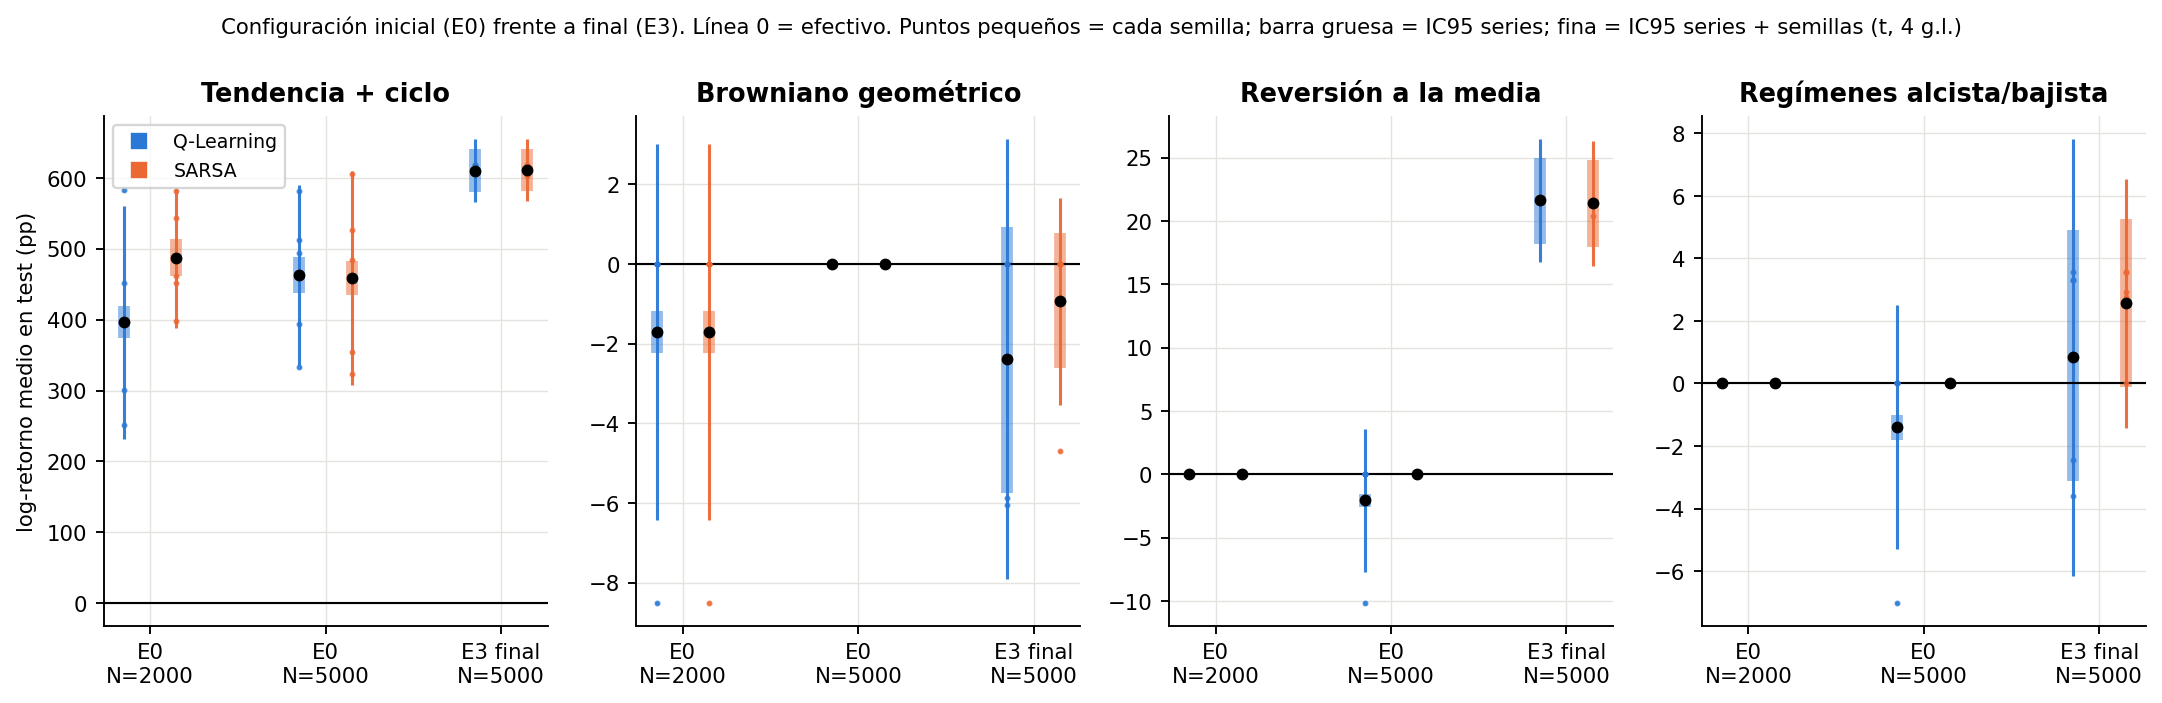
\includegraphics[width=0.94\textwidth]{fig1_inicial_vs_optimizada.png}
\caption{\textbf{Evolución:} configuración inicial (E0) frente a la final (E3), en test. La línea 0 es quedarse en efectivo.
En reversión y regímenes, E0 se queda clavado en 0: no opera. La final opera y, en reversión, supera claramente al efectivo.
Barra gruesa: IC95 por series; barra fina: IC95 por series y semillas. Puntos: cada semilla.}
\label{fig:evol}
\end{figure}

\begin{table}[h]
\centering
\caption{\textbf{Resultados en test} (100 series nuevas). Log-retorno medio en \% (media de 5 semillas, IC95 \emph{bootstrap} sobre series).
En \textbf{negrita}, lo que supera al efectivo con un IC que excluye el 0. Operaciones: media por serie. Episodios hasta convergencia: criterio de estabilización de la curva de validación (orientativo; ver §4).}
\label{tab:res}
\small
\begin{tabular}{lcccc}
\toprule
 & Tendencia + ciclo & Browniano & Reversión a la media & Regímenes \\
\midrule
Aleatorio & +145,2 & $-$20,8 & $-$15,7 & $-$28,3 \\
Buy \& Hold & +337,5 & $-$6,2 & $-$1,1 & $-$21,9 \\
Efectivo (no operar) & 0 & 0 & 0 & 0 \\
\midrule
\textcolor{ql}{\textbf{Q-Learning}} & \textbf{+610,4}\ic{580}{641} & $-$2,4\ic{$-$5,8}{0,9} & \textbf{+21,6}\ic{18,3}{25,2} & +0,8\ic{$-$3,2}{4,7} \\
\textcolor{sa}{\textbf{SARSA}}      & \textbf{+611,5}\ic{581}{642} & $-$0,9\ic{$-$2,6}{0,7} & \textbf{+21,4}\ic{18,0}{24,8} & +2,6\ic{$-$0,2}{5,4} \\
\midrule
Operaciones (Q-L / SARSA) & 62 / 53 & 0,4 / 0,2 & 52 / 45 & 33 / 28 \\
Episodios hasta convergencia & 500 / 500 & 200 / 200 & 2500 / 800 & 1000 / 1300 \\
$\alpha\cdot\gamma$ (Q-L \;|\; SARSA) & .005·.95 \;|\; .005·.90 & .001·.99 \;|\; .001·.99 & .002·.95 \;|\; .001·.95$^\ast$ & .001·.99 \;|\; .001·.99 \\
\bottomrule
\end{tabular}\\[1pt]
{\scriptsize $^\ast$\,SARSA-reversión con $\varepsilon=0{,}1$ constante; el resto, $\varepsilon$: 1\,$\to$\,0,01. Todos con $N=5000$ episodios.}
\end{table}

\begin{figure}[h]
\centering
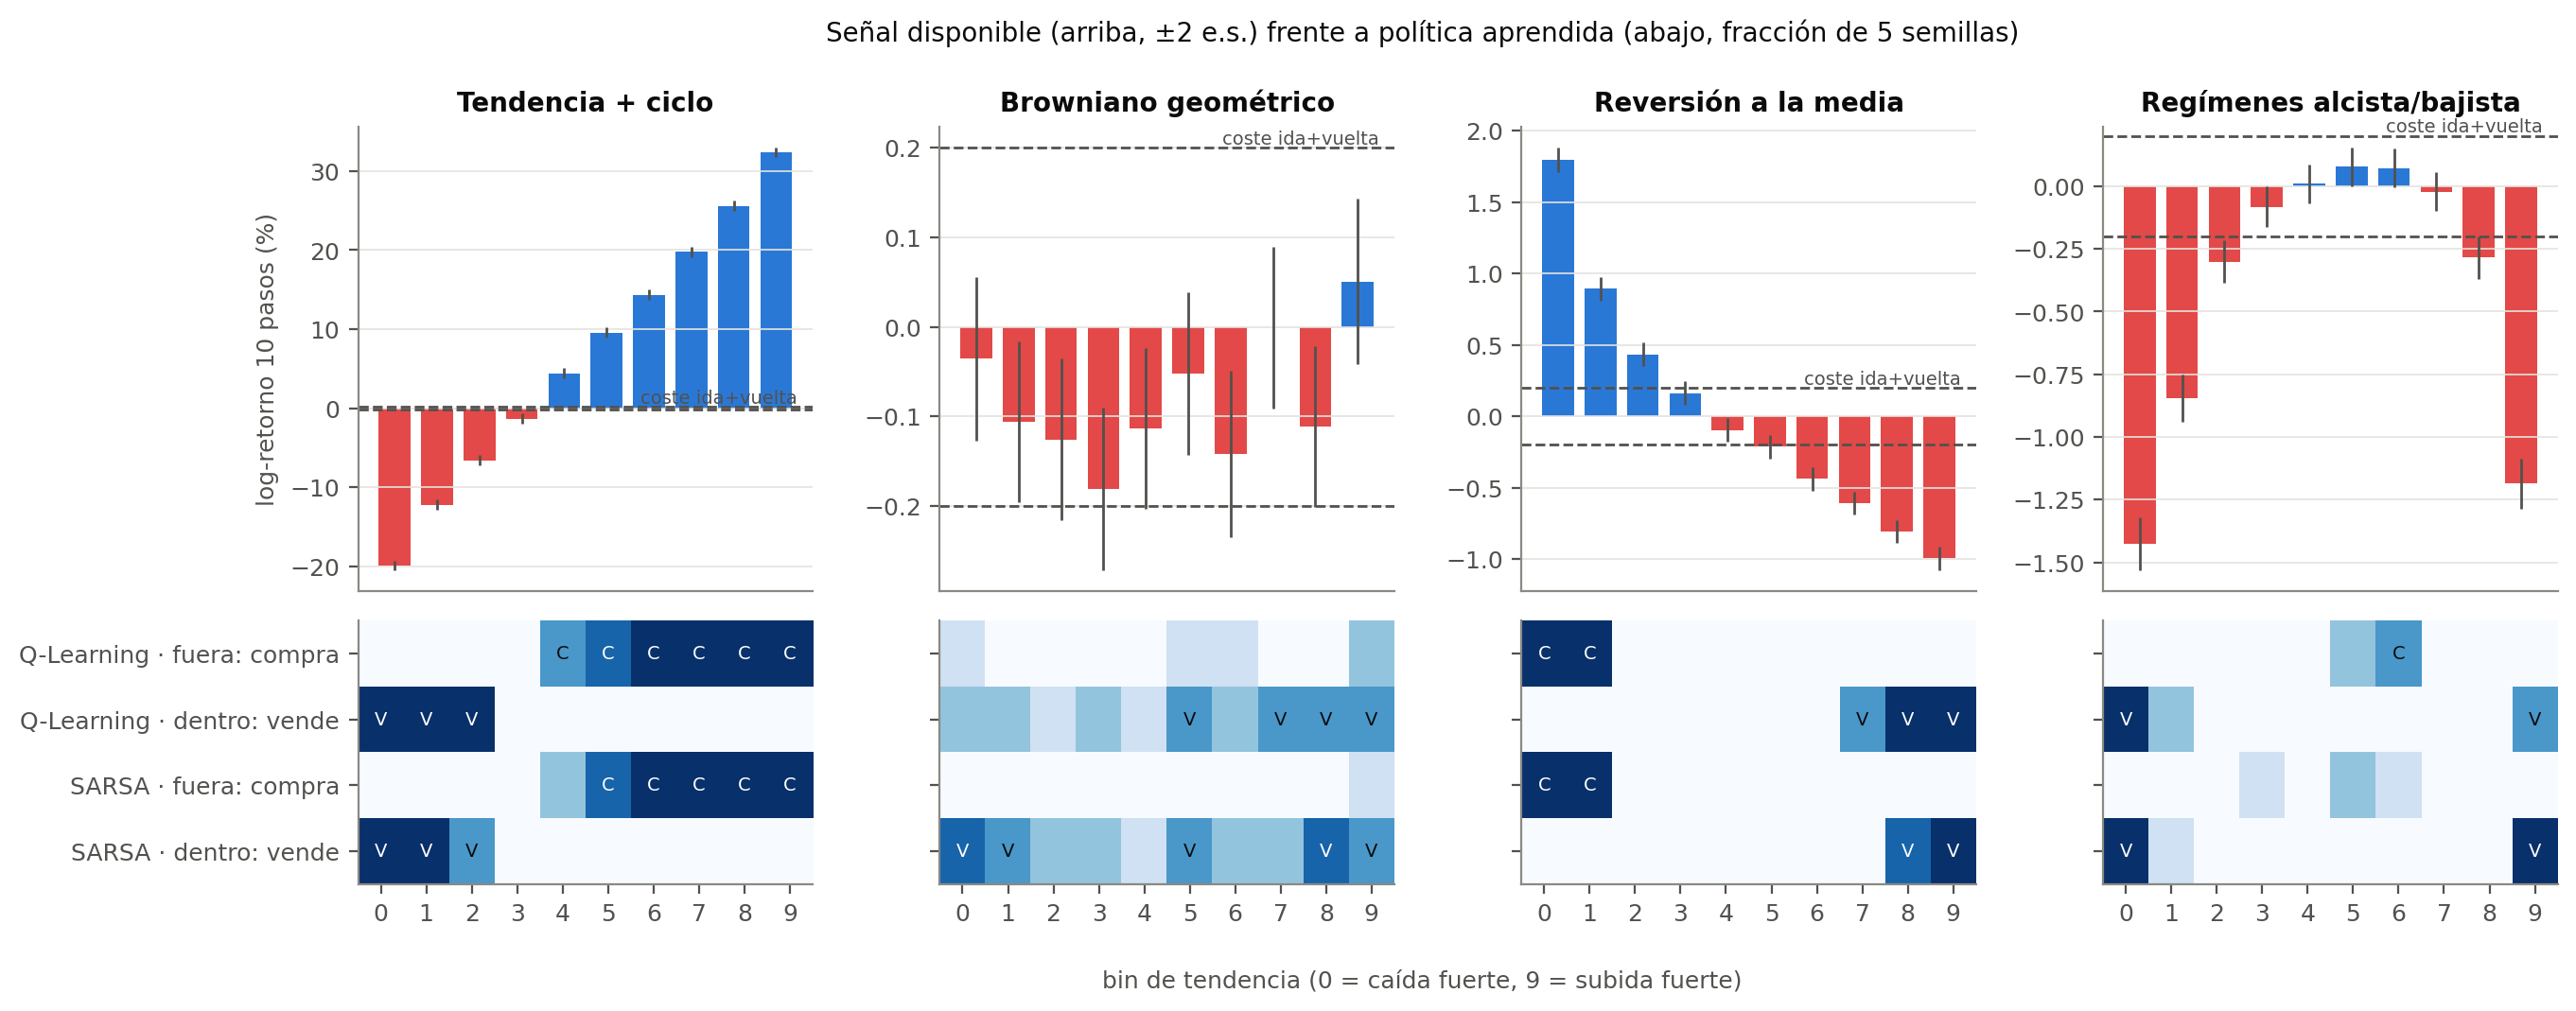
\includegraphics[width=0.94\textwidth]{fig_senal_politica.png}
\caption{\textbf{¿Tiene sentido lo aprendido?} Arriba: la \emph{señal real} de cada mercado (log-retorno de los 10 pasos siguientes según el bin de tendencia; líneas discontinuas: coste de comprar y vender).
Abajo: la \emph{política aprendida} (C = compra si está fuera, V = vende si está dentro; la intensidad indica cuántas de las 5 semillas coinciden).
La política reproduce la señal: \emph{momentum} en el cíclico, comprar en los bins 0--1 y vender en los 7--9 en reversión, prácticamente no comprar en el browniano y vender en los extremos en regímenes.}
\label{fig:senal}
\end{figure}

\begin{multicols}{2}

\sect{3. Lectura de los resultados}
\textbf{Donde hay señal, el agente la explota.} En reversión gana +21,6\,pp frente al efectivo y +22,7\,pp frente a Buy \& Hold, y la política es la de manual (Fig.~\ref{fig:senal}).
En el cíclico, +610\,pp: casi el doble que Buy \& Hold.

\textbf{Donde no hay señal, no opera.} En el browniano, lo racional es quedarse fuera, y es lo que hace (0,4 operaciones por serie). El $-$2,4 no se distingue del 0.

\textbf{Q-Learning $\approx$ SARSA.} Todas las diferencias Q$-$S tienen un IC que incluye el 0 (reversión: +0,2\ic{$-$1,8}{2,2}).
Q-Learning opera algo más, que es lo esperable de un objetivo \emph{off-policy}.

\sect{4. Análisis crítico}
\begin{itemize}
\item \textbf{Batir a Buy \& Hold no prueba que haya aprendido.} En regímenes, la configuración inicial, que \emph{no opera}, ya bate a Buy \& Hold por +21,9\,pp. Frente al efectivo, la ganancia (+0,8 y +2,6) no es significativa: su valor es \emph{evitar pérdidas}, no ganar dinero.
\item \textbf{El +610\,\% del cíclico} es una propiedad del generador (ruido del 10\,\% por paso) y del horizonte, no una rentabilidad realista.
\item \textbf{Convergencia.} La afirmación «SARSA converge antes» no es robusta: el orden depende del umbral elegido. Con hiperparámetros idénticos, SARSA es más rápido en 19 de 33 casos, pero solo 3 son significativos. Es una convergencia empírica, no garantizada.
\item \textbf{Recompensa $\neq$ métrica.} El entorno premia el retorno simple y nosotros medimos el log-retorno. En el browniano, Buy \& Hold suma $\sum r=+3{,}6$ y, sin embargo, $L=-6{,}2$.
\item \textbf{Limitaciones:} solo 5 semillas, y las series de test ya se habían inspeccionado durante el desarrollo, así que la reconstrucción de §2 es exploratoria.
\textbf{Reproducibilidad:} hay 1140 entrenamientos guardados (600 del ajuste y 540 de la reconstrucción), y 40 reentrenamientos coinciden \emph{bit a bit} con los originales.
\end{itemize}

\sect{5. Más allá: BTC-USD real}
Entrenamos con datos diarios de 2014 a 2020, seleccionamos en 2021--22 y probamos en 2023 a oct.\ 2026.
Q-Learning: +82\,\%$\pm$27 frente a +381\,\% de Buy \& Hold (Sharpe 0,69 frente a 1,12). En el año bajista 2022 pierde un 11\,\%, frente al 44\,\% de Buy \& Hold.
Está fuera del mercado el 67\,\% del tiempo y sus 288 operaciones cuestan $\approx$25\,\% del capital en comisiones.
Con una sola variable de tendencia de 6 días \textbf{no hay ventaja explotable}: BTC se parece al caso «browniano con deriva», no al de reversión.

\sect{Conclusiones}
\begin{enumerate}[label=\arabic*.]
\item El RL tabular recupera la estrategia óptima \emph{cuando la señal supera los costes}, y aprende a no operar cuando no la hay.
\item El hiperparámetro decisivo es $\alpha$: debe ser pequeño frente a la ventaja por paso. Más episodios no compensan un $\alpha$ demasiado alto.
\item Q-Learning y SARSA son indistinguibles en rendimiento. La comparación honesta es frente al \emph{efectivo}, no solo frente a Buy \& Hold.
\end{enumerate}

\end{multicols}
\end{document}
